\documentclass{article}

\usepackage{amsmath,amssymb,amsfonts,amscd,array,amsthm}
\usepackage{subcaption}
\usepackage{mathdots}

\usepackage{pgf,tikz}
    \usetikzlibrary{3d,patterns}
	\usetikzlibrary{arrows}
	\usetikzlibrary{shapes}
	\usetikzlibrary{shapes.geometric}
	\usetikzlibrary{patterns}
	\usetikzlibrary{calc}
	\usetikzlibrary{decorations.pathreplacing,decorations.markings}
	
\usepackage{pstricks}
 
\definecolor{orange}{RGB}{255,102,0}
\definecolor{ggreen}{RGB}{0,153,0}
\definecolor{darkblue}{RGB}{0,0,255}
\definecolor{purple}{RGB}{153,51,255}
\definecolor{turq}{RGB}{72,209,204}
\definecolor{gray}{RGB}{220,220,220}
\definecolor{rred}{rgb}{0.9, 0.17, 0.31}

\tikzset{arrow data/.style 2 args={%
      decoration={%
         markings,
         mark=at position #1 with \arrow{#2}},
         postaction=decorate}
      }%

\newcommand\heapblock[4]{\fill[fill=#4, fill opacity=0.35, draw=#4, line width=1.1pt, rounded corners,shift={(\xxaxis:#1)},shift={(\yyaxis:#2)}] (-1,-1) rectangle (1,1);\node at (#1,#2) {\footnotesize $#3$};}
\newcommand\dheapblock[4]{\draw[dotted, draw=#4, line width=1.1pt, rounded corners,shift={(\xxaxis:#1)},shift={(\yyaxis:#2)}] (-1,-1) rectangle (1,1);\node at (#1,#2) {\footnotesize $#3$};}

\newcommand\xxaxis{0}
\newcommand\yyaxis{90}
%\newcommand\sq[2]{
%    \fill[fill=gray!30, draw=black, rounded corners, line width=1pt, shift={(\xxaxis:#1)}, shift={(\yyaxis:#2)}] 
%    (0,0) -- (1,0) -- (1,-1) -- (0,-1) -- cycle; }
%
%\newcommand\sqor[2]{
%    \fill[draw=orange, fill=orange!10, line width=1.1pt, rounded corners, shift={(\xxaxis:#1)}, shift={(\yyaxis:#2)}]
%    (0,0) -- (1,0) -- (1,-1) -- (0,-1) -- cycle; }
%\newcommand\sqorhash[2]{
%    \fill[pattern=north east lines, pattern color=orange!35, draw=orange, line width=1.1pt, rounded corners, shift={(\xxaxis:#1)}, shift={(\yyaxis:#2)}]
%    (0,0) -- (1,0) -- (1,-1) -- (0,-1) -- cycle; }
%\newcommand\sqorcheck[2]{
%    \fill[pattern=checkerboard, pattern color=orange!06, draw=orange, line width=1.1pt, rounded corners, shift={(\xxaxis:#1)}, shift={(\yyaxis:#2)}]
%    (0,0) -- (1,0) -- (1,-1) -- (0,-1) -- cycle; }
%
%\newcommand\sqgr[2]{
%    \fill[draw=ggreen, fill=ggreen!05, line width=1.1pt, rounded corners, shift={(\xxaxis:#1)}, shift={(\yyaxis:#2)}]
%    (0,0) -- (1,0) -- (1,-1) -- (0,-1) -- cycle; }
%\newcommand\sqgrhash[2]{
%    \fill[pattern=north east lines, pattern color=ggreen!35, draw=ggreen, line width=1.1pt, rounded corners, shift={(\xxaxis:#1)}, shift={(\yyaxis:#2)}]
%    (0,0) -- (1,0) -- (1,-1) -- (0,-1) -- cycle; }
%\newcommand\sqgrcheck[2]{
%    \fill[pattern=checkerboard, pattern color=ggreen!06, draw=ggreen, line width=1.1pt, rounded corners, shift={(\xxaxis:#1)}, shift={(\yyaxis:#2)}]
%    (0,0) -- (1,0) -- (1,-1) -- (0,-1) -- cycle; }
%
%\newcommand\sqp[2]{
%    \fill[draw=purple, fill=purple!08, line width=1.1pt, rounded corners, shift={(\xxaxis:#1)}, shift={(\yyaxis:#2)}]
%    (0,0) -- (1,0) -- (1,-1) -- (0,-1) -- cycle; }
%\newcommand\sqphash[2]{
%    \fill[pattern=north east lines, pattern color=purple!35, draw=purple, line width=1.1pt, rounded corners, shift={(\xxaxis:#1)}, shift={(\yyaxis:#2)}]
%    (0,0) -- (1,0) -- (1,-1) -- (0,-1) -- cycle; }
%\newcommand\sqpcheck[2]{
%    \fill[pattern=checkerboard, pattern color=purple!06, draw=purple, line width=1.1pt, rounded corners, shift={(\xxaxis:#1)}, shift={(\yyaxis:#2)}]
%    (0,0) -- (1,0) -- (1,-1) -- (0,-1) -- cycle; }
%
%\newcommand\sqbl[2]{
%    \fill[draw=darkblue, fill=darkblue!05, line width=1.1pt, rounded corners, shift={(\xxaxis:#1)}, shift={(\yyaxis:#2)}]
%    (0,0) -- (1,0) -- (1,-1) -- (0,-1) -- cycle; }
%\newcommand\sqblhash[2]{
%    \fill[pattern=north east lines, pattern color=darkblue!35, draw=darkblue, line width=1.1pt, rounded corners, shift={(\xxaxis:#1)}, shift={(\yyaxis:#2)}]
%    (0,0) -- (1,0) -- (1,-1) -- (0,-1) -- cycle; }
%\newcommand\sqblcheck[2]{
%    \fill[pattern=checkerboard, pattern color=darkblue!06, draw=darkblue, line width=1.1pt, rounded corners, shift={(\xxaxis:#1)}, shift={(\yyaxis:#2)}]
%    (0,0) -- (1,0) -- (1,-1) -- (0,-1) -- cycle; }
%    
%\newcommand\sqm[2]{
%    \fill[draw=magenta, fill=magenta!08, line width=1.1pt, rounded corners, shift={(\xxaxis:#1)}, shift={(\yyaxis:#2)}]
%    (0,0) -- (1,0) -- (1,-1) -- (0,-1) -- cycle; }
%\newcommand\sqmhash[2]{
%    \fill[pattern=north east lines, pattern color=magenta!35, draw=magenta, line width=1.1pt, rounded corners, shift={(\xxaxis:#1)}, shift={(\yyaxis:#2)}]
%    (0,0) -- (1,0) -- (1,-1) -- (0,-1) -- cycle; }
%
%% The empty square
%\newcommand\bsq[2]{
%    \fill[fill=white, dotted, draw=black, line width=0.5pt, rounded corners, shift={(\xxaxis:#1)},shift={(\yyaxis:#2)}]
%    (0.05,-0.05) -- (0.95,-0.05) -- (0.95,-0.95) -- (0.05,-0.95) -- cycle; }

%% Kirsten's code %%

% The square
 

\newcommand\nsq[3]{

  \fill[fill=cyan!30, draw=black, rounded corners, line width=1pt, shift={(\xxaxis:#1)},shift={(\yyaxis:#2)}] (0,0) -- (2,0) -- (2,-2) -- (0,-2) --cycle;
      \node at (#1+1,#2-1) {$#3$};
}

% colored square
\newcommand\csq[2]{
  \fill[fill=magenta, draw=black,rounded corners, shift={(\xxaxis:#1)},shift={(\yyaxis:#2)}] (0,0) -- (1,0) -- (1,-1) -- (0,-1) --(0,0);
}

% The empty square
\newcommand\bsq[2]{
  \fill[fill=white, fill opacity=0.5, densely dashed, draw=black, rounded corners, shift={(\xxaxis:#1)},shift={(\yyaxis:#2)}] (0,0) -- (1,0) -- (1,-1) -- (0,-1) --(0,0);
<<<<<<< HEAD
}


\begin{document}


Heap Adventures\\
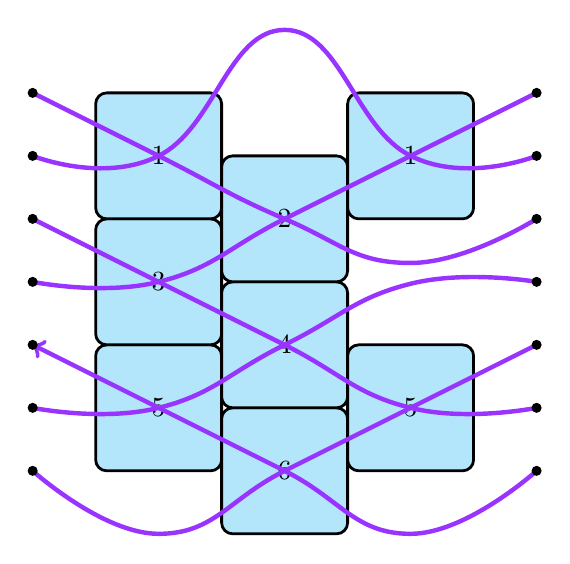
\begin{tikzpicture}[scale=0.8]
\nsq{0}{0}{5};
\nsq{0}{2}{3};
\nsq{0}{4}{1};
\nsq{2}{-1}{6};
\nsq{2}{1}{4};
\nsq{2}{3}{2};
\nsq{4}{0}{5};
\nsq{4}{4}{1};


%\node at (7.1,4) {$1$};
%\node at (7.1,3) {$2$};
%\node at (7.1,2) {$3$};
%\node at (7.1,1) {$4$};
%\node at (7.1,0) {$5$};
%\node at (7.1,-1) {$6$};
%\node at (7.1,-2) {$7$};
%
%\node at (-1.1,4) {$1$};
%\node at (-1.1,3) {$2$};
%\node at (-1.1,2) {$3$};
%\node at (-1.1,1) {$4$};
%\node at (-1.1,0) {$5$};
%\node at (-1.1,-1) {$6$};
%\node at (-1.1,-2) {$7$};

\draw [purple,ultra thick] plot [smooth, tension=0.8] coordinates {(7,4)(5,3)(3,2)(1,1)(-1,1)};
\draw [purple,ultra thick] plot [smooth, tension=0.8] coordinates {(7,3)(5,3)(3,5)(1,3)(-1,3)};
\draw [purple,ultra thick] plot [smooth, tension=0.8] coordinates {(7,2)(5,1.3)(3,2)(1,3)(-1,4)};
\draw [purple,ultra thick] plot [smooth, tension=0.8] coordinates {(7,1)(5,.97)(3,0)(1,-1)(-1,-1)};
\draw [purple,ultra thick] plot [smooth, tension=0.8] coordinates {(7,0)(5,-1)(3,-2)(1,-3)(-1,-2)};
\draw [purple,ultra thick] plot [smooth, tension=0.8] coordinates {(7,-1)(5,-1)(3,0)(1,1)(-1,2)};
\draw [purple,ultra thick, ->] plot [smooth, tension=0.8] coordinates {(7,-2)(5,-3)(3,-2)(1,-1)(-1,0)};


\draw[fill=black] \foreach \y in {-2,-1,0,1,2,3,4} {(-1,\y) circle (2pt)};
\draw[fill=black] \foreach \y in {-2,-1,0,1,2,3,4} {(7,\y) circle (2pt)};

\end{tikzpicture}

\vspace{-5.7cm}


\hspace{7cm}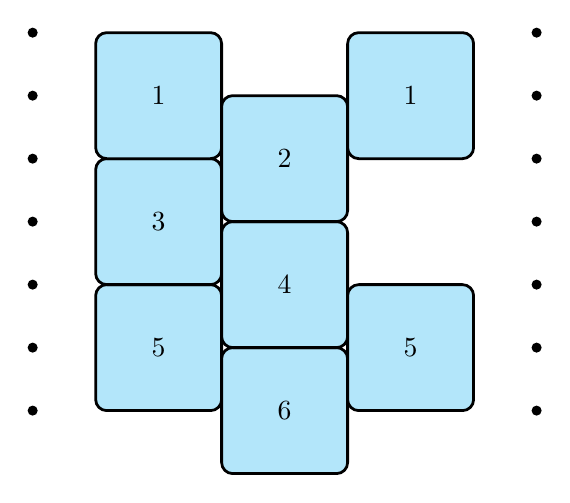
\begin{tikzpicture}[scale=0.8]
\nsq{0}{0}{5};
\nsq{0}{2}{3};
\nsq{0}{4}{1};
\nsq{2}{-1}{6};
\nsq{2}{1}{4};
\nsq{2}{3}{2};
\nsq{4}{0}{5};
\nsq{4}{4}{1};


\node at (0,0){%
\psset{unit=.8cm}
\pscurve[linecolor=purple,linewidth=2pt]{-}(7,4)(5,3)(3,2)(1,1)(-1,1)

\pscurve[linecolor=purple,linewidth=2pt]{-}(7,3)(5,3)(3,5)(1,3)(-1,3)

\pscurve[linecolor=purple,linewidth=2pt]{-}(7,2)(3,2)(1,3)(-1,4)

\pscurve[linecolor=purple,linewidth=2pt]{-}(7,1)(3,0)(1,-1)(-1,-1)

\pscurve[linecolor=purple,linewidth=2pt]{-}(7,0)(5,-1)(3,-2)(-1,-2)

\pscurve[linecolor=purple,linewidth=2pt]{-}(7,-1)(5,-1)(3,0)(1,1)(-1,2)

\pscurve[linecolor=purple,linewidth=2pt]{-}(7,-2)(3,-2)(1,-1)(-1,0)
};

\draw[fill=black] \foreach \y in {-2,-1,0,1,2,3,4} {(-1,\y) circle (2pt)};
\draw[fill=black] \foreach \y in {-2,-1,0,1,2,3,4} {(7,\y) circle (2pt)};

%\filldraw[purple] (4.5,1.5) circle (5pt);
%\filldraw[white] (3,0.5) circle (5pt);
%\filldraw[purple] (1.5,1.5) circle (5pt);
%\filldraw[purple] (3,2.5) circle (5pt);
%\filldraw[purple] (3,4.5) circle (5pt);
%\filldraw[purple] (1.5,3.5) circle (5pt);

\end{tikzpicture}

%\newpage
%String Diagram Adventures\\
%
%\begin{tikzpicture}[scale=0.8]
%%\nsq{0}{0}{5};
%%\nsq{0}{2}{3};
%%\nsq{0}{4}{1};
%%\nsq{2}{-1}{6};
%%\nsq{2}{1}{4};
%%\nsq{2}{3}{2};
%%\nsq{4}{0}{5};
%%\nsq{4}{4}{1};
%
%
%%\node at (7.1,4) {$1$};
%%\node at (7.1,3) {$2$};
%%\node at (7.1,2) {$3$};
%%\node at (7.1,1) {$4$};
%%\node at (7.1,0) {$5$};
%%\node at (7.1,-1) {$6$};
%%\node at (7.1,-2) {$7$};
%%
%%\node at (-1.1,4) {$1$};
%%\node at (-1.1,3) {$2$};
%%\node at (-1.1,2) {$3$};
%%\node at (-1.1,1) {$4$};
%%\node at (-1.1,0) {$5$};
%%\node at (-1.1,-1) {$6$};
%%\node at (-1.1,-2) {$7$};
%
%%\draw [red,arrow data={0.25}{stealth},
%%           arrow data={0.5}{stealth},
%%           arrow data={0.75}{stealth}] plot [smooth,tension=1];
%
%%\draw [purple,ultra thick] plot [smooth, tension=0.8] coordinates {(7,4)(5,3)(3,2)(1,1)(-1,1)};
%%\draw [purple,ultra thick] plot [smooth, tension=0.8] coordinates {(7,3)(5,3)(3,5)(1,3)(-1,3)};
%%\draw [purple,ultra thick] plot [smooth, tension=0.8] coordinates {(7,2)(5,1.3)(3,2)(1,3)(-1,4)};
%%\draw [purple,ultra thick] plot [smooth, tension=0.8] coordinates {(7,1)(5,.97)(3,0)(1,-1)(-1,-1)};
%
%[
%    triangle/.style = {fill=blue!20, regular polygon, regular polygon sides=3 },
%    node rotated/.style = {rotate=180},
%    border rotated/.style = {shape border rotate=180}
%  ]
%\node [draw, purple, triangle,fill=purple] at (1,-3){};
%\draw [purple,ultra thick] plot [smooth, tension=0.8] coordinates {(7,0)(5,-1)(3,-2)(1,-3)};
%\draw [purple,ultra thick] plot [smooth, tension=0.8] coordinates {(7,-1)(5,-1)(3,0)(1,1)(-1,2)};
%\draw [purple,ultra thick] plot [smooth, tension=0.8] coordinates {(7,-2)(5,-3)(3,-2)(1,-1)(-1,0)};
%
%%\draw[fill=black] \foreach \y in {-2,-1,0,1,2,3,4} {(-1,\y) circle (2pt)};
%\draw[fill=black] \foreach \y in {-2,-1,0,1,2,3,4} {(7,\y) circle (2pt)};
%
%\end{tikzpicture}
%
%
%%\begin{center} \begin{tikzpicture}
%%    \sqbl{0}{9};    \node at (0.5,8.5)   {\scalebox{0.85}{$1$}};
%%    \sqbl{0.5}{8};  \node at (1,7.5)     {\scalebox{0.85}{$2$}};
%%                    \node at (1.8,6.6)   {$\ddots$};
%%    \sqbl{2}{6};    \node at (2.5,5.5)   {\scalebox{0.85}{$k$}};
%%    \sqbl{3}{6};    \node at (3.5,5.5)   {\scalebox{0.85}{$k+2$}};
%%    \sqbl{3.5}{5};  \node at (4,4.5)     {\scalebox{0.85}{$k+3$}};
%%                    \node at (4.8,3.65)  {$\ddots$};
%%    \sqbl{5}{3};    \node at (5.5,2.5)   {\scalebox{0.85}{$k'$}};
%%    \sqbl{5.5}{2};  \node at (6,1.5)     {\scalebox{0.85}{$k'+1$}};
%%
%%    \sqor{2.5}{7};  \node at (3,6.5)     {\scalebox{0.85}{$k+1$}};
%%                    \node at (2.25,7.6)  {$\ddots$};
%%    \sqor{1}{9};    \node at (1.5,8.5)   {\scalebox{0.85}{$3$}};
%%    \sqor{0.5}{10}; \node at (1,9.5)     {\scalebox{0.85}{$2$}};
%%    \sqor{0}{11};   \node at (0.5,10.5)  {\scalebox{0.85}{$1$}};
%%    \sqor{3}{8};    \node at (3.5,7.5)   {\scalebox{0.85}{$k+2$}};
%%                    \node at (2.75,8.6)  {$\ddots$};
%%    \sqor{1.5}{10}; \node at (2,9.5)     {\scalebox{0.85}{$4$}};
%%    \sqor{1}{11};   \node at (1.5,10.5)  {\scalebox{0.85}{$3$}};
%%    \sqor{0.5}{12}; \node at (1,11.5)    {\scalebox{0.85}{$2$}};
%%                    \node at (2,12.5)    {$\iddots$};
%%                    \node at (4.5,8.5)   {$\iddots$};
%%                    \node at (3,11.5)    {$\iddots$};
%%                    \node at (5.1,11.6)  {$\ddots$};
%%                    \node at (4,10.5)    {$\cdots$};
%%                    \node at (4,9.5)     {$\cdots$};
%%    \sqor{3}{14};   \node at (3.5,13.5)  {\scalebox{0.85}{$m+1$}};
%%    \sqor{3.5}{13}; \node at (4,12.5)    {\scalebox{0.85}{$m+2$}};
%%    \sqor{5.5}{11}; \node at (6,10.5)    {\scalebox{0.85}{$k'+1$}};
%%    \sqor{5}{10};   \node at (5.5,9.5)   {\scalebox{0.85}{$k'$}};
%%    
%%    \sqgr{2.5}{5};  \node at (3,4.5)     {\scalebox{0.85}{$k+1$}};
%%    \sqgr{2}{4};    \node at (2.5,3.5)   {\scalebox{0.85}{$k$}};
%%    \sqgr{3}{4};    \node at (3.5,3.5)   {\scalebox{0.85}{$k+2$}};
%%                    
%%    \sqgr{4.5}{2};  \node at (5,1.5)     {\scalebox{0.85}{$k'-1$}};
%%    \sqgr{5}{1};    \node at (5.5,0.5)   {\scalebox{0.85}{$k'$}};
%%                    \node at (4.8,-1)    {$\iddots$};
%%    \sqgr{0.5}{2};  \node at (1,1.5)     {\scalebox{0.85}{$2$}};
%%    \sqgr{0}{1};    \node at (0.5,0.5)   {\scalebox{0.85}{$1$}};
%%    \sqgr{1}{1};    \node at (1.5,0.5)   {\scalebox{0.85}{$3$}};
%%    \sqgr{0.5}{0};  \node at (1,-0.5)    {\scalebox{0.85}{$2$}};
%%    \sqgr{1.5}{2};  \node at (2,1.5)     {\scalebox{0.85}{$4$}};
%%                    \node at (2,-1.5)    {$\ddots$};
%%    \sqgr{3}{-2};   \node at (3.5,-2.5)  {\scalebox{0.85}{$m+1$}};
%%                    \node at (1.8,2.5)   {$\iddots$};
%%                    \node at (2.8,2.5)   {$\iddots$};
%%                    \node at (3.5,1.5)   {$\cdots$};
%%                    \node at (3.5,0.5)   {$\cdots$};
%%                    \node at (3.5,-0.5)  {$\cdots$};
%%                    \node at (4.3,2.5)   {$\ddots$};
%%\end{tikzpicture} \end{center}
%%
%%\pagebreak
%%
%%\begin{figure}[h!] \centering \begin{tikzpicture}%[scale=0.85]
%%    \sqor{0}{10};       \node at (0.5,9.5) {\footnotesize $3$};
%%    \sqor{0.5}{9};      \node at (1,8.5)   {\footnotesize $4$};
%%    \sqor{1}{8};        \node at (1.5,7.5) {\footnotesize $5$};
%%    \sqor{1.5}{7};      \node at (2,6.5)   {\footnotesize $6$};
%%    \sqorhash{2}{6};    \node at (2.5,5.5) {\footnotesize $7$};
%%    \sqbl{0}{8};        \node at (0.5,7.5) {\footnotesize $3$};
%%    \sqbl{0.5}{7};      \node at (1,6.5)   {\footnotesize $4$};
%%    \sqbl{1}{6};        \node at (1.5,5.5) {\footnotesize $5$};
%%    \sqblhash{1.5}{5};  \node at (2,4.5)   {\footnotesize $6$};
%%    \sqgrhash{2}{4};    \node at (2.5,3.5) {\footnotesize $7$};
%%    \sqgrhash{1.5}{3};  \node at (2,2.5)   {\footnotesize $6$};
%%    \sqgr{1}{2};        \node at (1.5,1.5) {\footnotesize $5$};
%%    \sqgr{0.5}{1};      \node at (1,0.5)   {\footnotesize $4$};
%%    \sqgr{0}{0};        \node at (0.5,-0.5){\footnotesize $3$};
%%\end{tikzpicture}
%%\caption{}\label{fig:slideexheap1}
%%\end{figure}
%%
%
%%\begin{tikzpicture}
%%
%%\draw[step=1cm,color=gray] (0,0) grid (3,3);    
%%\draw[draw=black,solid, -triangle 90,fill=black] (0,0) -- (0,3);
%%
%%\end{tikzpicture}

\newpage
Experiments for Thesis $\ldots$\\
\bigskip
Example 1.4.1\\
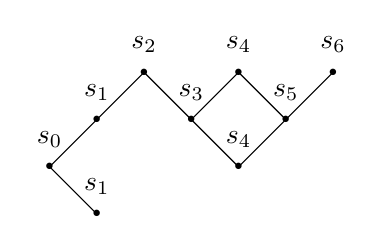
\begin{tikzpicture}[scale=0.6]
	\node[scale=0.6, label=above:$s_{2}$] at (2,5.5) {$\bullet$};
	\node[scale=0.6, label=above:$s_{4}$] at (4,5.5) {$\bullet$};
	\node[scale=0.6, label=above:$s_{6}$] at (6,5.5) {$\bullet$};
	\node[scale=0.6, label=above:$s_{1}$] at (1,4.5) {$\bullet$};
	\node[scale=0.6, label=above:$s_{3}$] at (3,4.5) {$\bullet$};
	\node[scale=0.6, label=above:$s_{5}$] at (5,4.5) {$\bullet$};
	\node[scale=0.6, label=above:$s_{0}$] at (0,3.5) {$\bullet$};
	\node[scale=0.6, label=above:$s_{4}$] at(4,3.5) {$\bullet$};
	\node[scale=0.6, label=above:$s_{1}$] at (1,2.5) {$\bullet$};
\draw (1,2.5)--(0,3.5)--(1,4.5)--(2,5.5)--(3,4.5)--(4,3.5);
\draw (3,4.5)--(4,5.5)--(5,4.5)--(4,3.5);
\draw (6,5.5)--(5,4.5);
\end{tikzpicture}


Example 1.4.2\\
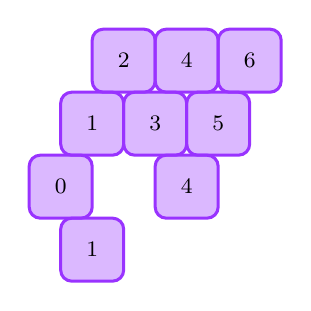
\begin{tikzpicture}[scale=0.4]
\heapblock{2}{6}{2}{purple}
\heapblock{4}{6}{4}{purple}
\heapblock{6}{6}{6}{purple}
\heapblock{1}{4}{1}{purple}
\heapblock{3}{4}{3}{purple}
\heapblock{5}{4}{5}{purple}
\heapblock{0}{2}{0}{purple}
\heapblock{4}{2}{4}{purple}
\heapblock{1}{0}{1}{purple}
\end{tikzpicture}

Example 1.4.3\\
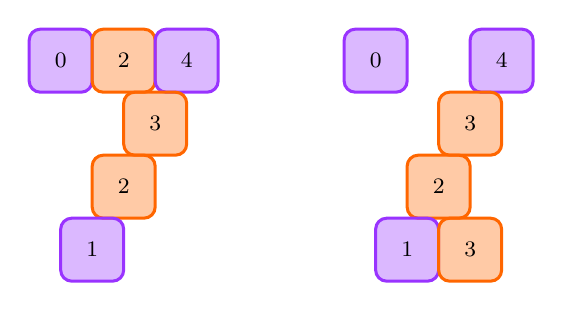
\begin{tikzpicture}[scale=0.4]
\heapblock{0}{6}{0}{purple}
\heapblock{2}{6}{2}{orange}
\heapblock{4}{6}{4}{purple}	
\heapblock{3}{4}{3}{orange}
\heapblock{2}{2}{2}{orange}
\heapblock{1}{0}{1}{purple}

\heapblock{10}{6}{0}{purple}
\heapblock{14}{6}{4}{purple}
\heapblock{13}{4}{3}{orange}
\heapblock{12}{2}{2}{orange}
\heapblock{11}{0}{1}{purple}
\heapblock{13}{0}{3}{orange}
\end{tikzpicture}

\newpage
Finite Irreducible Coxeter Graphs Figure
\begin{figure}[h!]
\begin{tabular}{m{7cm} m{7cm}}
\begin{subfigure}{0.5\textwidth} \centering
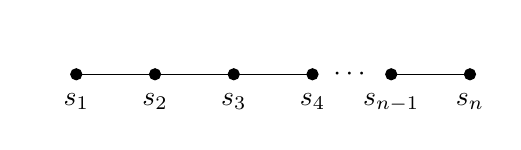
\begin{tikzpicture}[scale=1.0]%A_{n}
\draw[fill=black] \foreach \x in {1,2,...,6} {(\x,10) circle (2pt)};
\draw {(.5,10) node{}
(1.5,10) node[label=above:\textcolor{white}{$4$}]{}
(4.5,10) node{$\cdots$}
(1,10) node[label=below:$s_1$]{}
(2,10) node[label=below:$s_2$]{}
(3,10) node[label=below:$s_3$]{}
(4,10) node[label=below:$s_4$]{}
(5,10) node[label=below:$s_{n-1}$]{}
(6,10) node[label=below:$s_{n}$]{}
[-] (1,10) -- (4,10)
[-] (5,10) -- (6,10)
(1,10) node{}}; 
\end{tikzpicture}
\caption{$A_{n}$} \label{fig:A}
\end{subfigure} &

\begin{subfigure}{0.5\textwidth} \centering
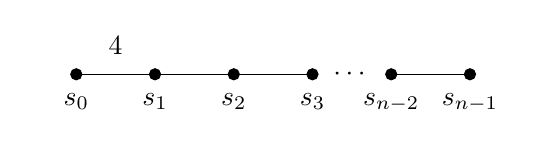
\begin{tikzpicture}[scale=1.0]%B_{n}
\draw [fill=black] \foreach \x in {1,2,...,6} {(\x,8.5) circle (2pt)};
\draw {(.5,8.5) node{}
(1.5,8.5) node[label=above:$4$]{}
(4.5,8.5) node{$\cdots$}
(1,8.5) node[label=below:$s_0$]{}
(2,8.5) node[label=below:$s_1$]{}
(3,8.5) node[label=below:$s_2$]{}
(4,8.5) node[label=below:$s_3$]{}
(5,8.5) node[label=below:$s_{n-2}$]{}
(6,8.5) node[label=below:$s_{n-1}$]{}
[-] (1,8.5) -- (4,8.5)
[-] (5,8.5) -- (6,8.5)
(2,8.5) node{}}; 
\end{tikzpicture}
\caption{$B_{n}$} \label{fig:B}
\end{subfigure} \\

    & \\ 

\begin{subfigure}{0.5\textwidth} \centering
\begin{tikzpicture}[scale=1.0]
\draw[fill=black] \foreach \x in {1,2} {(\x,0) circle (2pt)};
\fill[fill=white] (2,1) circle (2pt);
\draw {(.25,0) node{}
(1.5,0) node[label=above:$m$]{}
[-] (1,0) -- (2,0)
(2,0) node{}};
\end{tikzpicture}
\caption{$I_{2}(m)$} \label{fig:I}
\end{subfigure} &

\begin{subfigure}{0.5\textwidth} \centering
\begin{tikzpicture}[scale=1.0]
\draw[fill=black] \foreach \x in {1,2,...,6} {(\x,6.5) circle (2pt)};%D_{n}
\draw[fill=black] (2,7.5) circle (2pt);
\draw {(.5,6.5) node{}
(4.5,6.5) node{$\cdots$}
[-] (1,6.5) -- (4,6.5)
[-] (5,6.5) -- (6,6.5)
[-] (2,6.5) -- (2,7.5)
(2,6.5) node{}};
\end{tikzpicture}
\caption{$D_{n}$} \label{fig:D}
\end{subfigure} \\

    & \\ 
    
\begin{subfigure}{0.5\textwidth} \centering
\begin{tikzpicture}[scale=1.0]%E_{6}
\draw[fill=black] \foreach \x in {1,2,...,5} {(\x,4.5) circle (2pt)};
\draw[fill=black] (3,5.5) circle (2pt);
\draw {
[-] (1,4.5) -- (5,4.5)
[-] (3,4.5) -- (3,5.5)
(3,4.5) node{}};
\end{tikzpicture}
\caption{$E_{6}$} \label{fig:E6}
\end{subfigure} &



\begin{subfigure}{0.5\textwidth} \centering
\begin{tikzpicture}[scale=1.0]%E_{7}
\draw[fill=black] \foreach \x in {1,2,...,6} {(\x,4.5) circle (2pt)};
\draw[fill=black] (3, 5.5) circle (2pt);
\draw {
[-] (1,4.5) -- (5,4.5)
[-] (5,4.5) -- (6,4.5)
[-] (3,4.5) -- (3,5.5)
(3,4.5) node{}};
\end{tikzpicture}
\caption{$E_{7}$} \label{fig:E7}
\end{subfigure} \\

    & \\ 


\begin{subfigure}{0.5\textwidth} \centering
\begin{tikzpicture}[scale=1.0]%E_{8}
\draw[fill=black] \foreach \x in {1,2,...,7} {(\x,4.5) circle (2pt)};
\draw[fill=black] (3,5.5) circle (2pt);
\draw {
[-] (1,4.5) -- (7,4.5)
[-] (3,4.5) -- (3,5.5)
(3,4.5) node{}};
\end{tikzpicture}
\caption{$E_{8}$} \label{fig:E6}
\end{subfigure} &

\begin{subfigure}{0.5\textwidth} \centering
\begin{tikzpicture}[scale=1.0]%F_{4}
\draw[fill=black] \foreach \x in {1,2,...,4} {(\x,3) circle (2pt)};
\fill[white] (1,4) circle (2pt);
\draw {(.5,3) node{}
(2.5,3) node[label=above:$4$]{}
[-] (1,3) -- (4,3)
(3,3) node{}};
\end{tikzpicture}
\caption{$F_{4}$} \label{fig:F4}
\end{subfigure} \\

&\\

\begin{subfigure}{0.5\textwidth} \centering
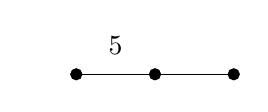
\begin{tikzpicture}[scale=1.0]
\draw[fill=black] \foreach \x in {1,2,...,3} {(\x,1.5) circle (2pt)};%H_{3}
\draw {(.5,1.5) node{}
(1.5,1.5) node[label=above:$5$]{}
[-] (1,1.5) -- (3,1.5)
(2,1.5) node{}}; 
\end{tikzpicture}
\caption{$H_{3}$} \label{fig:H}
\end{subfigure} &

\begin{subfigure}{0.5\textwidth} \centering
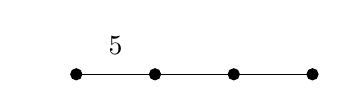
\begin{tikzpicture}[scale=1.0]
\draw[fill=black] \foreach \x in {1,2,...,4} {(\x,1.5) circle (2pt)};%H_{4}
\draw {(.5,1.5) node{}
(1.5,1.5) node[label=above:$5$]{}
[-] (1,1.5) -- (4,1.5)
(2,1.5) node{}}; 
\end{tikzpicture}
\caption{$H_{4}$} \label{fig:H}
\end{subfigure}
\end{tabular}
\caption{Coxeter graphs corresponding to the finite Coxeter groups.}
\label{fig:fincoxgraphs}
\end{figure}

\newpage
Affine Coxeter Graphs Figure
\begin{figure}[h!]
\begin{tabular}{m{7cm} m{7cm}}
\begin{subfigure}{0.5\textwidth} \centering
\begin{tikzpicture}[scale=1.0]%\widetilde{A}_{2}
\draw[fill=black] \foreach \x in {1,2} {(\x,10) circle (2pt)};
\fill[white] (1,11) circle (2pt);
\draw { (.5,10) node{}
(1.5,10) node[label=above:$\infty$]{}
[-] (1,10) -- (2,10)
(1,10) node{}}; 
\end{tikzpicture}
\caption{$\widetilde{A}_{2}$} \label{fig:affA2}
\end{subfigure} &

\begin{subfigure}{0.5\textwidth} \centering
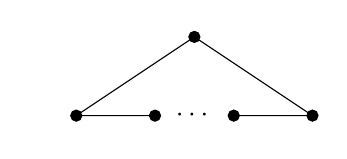
\begin{tikzpicture}[scale=1.0]%\widetilde{A}_{n}
\draw [fill=black] \foreach \x in {1,...,4} {(\x,7.5) circle (2pt)};
\draw [fill=black] (2.5, 8.5) circle (2pt);
\draw {(.5,8.5) node{}
(2.5,7.5) node{$\cdots$}
[-] (2.5,8.5) -- (1, 7.5)
[-] (2.5,8.5) -- (4, 7.5)
[-] (1,7.5) -- (2,7.5)
[-] (3,7.5) -- (4,7.5)
(2,8.5) node{}}; 
\end{tikzpicture}
\caption{$\widetilde{A}_{n}$} \label{fig:affAn}
\end{subfigure} \\

    & \\ 

\begin{subfigure}{0.5\textwidth} \centering
\begin{tikzpicture}[scale=1.0]%\widetilde{B}_{n}
\draw[fill=black] \foreach \x in {1,2,...,6} {(\x,0) circle (2pt)};
\draw[fill=black] (2,1) circle (2pt);
\draw {(.25,0) node{}
(5.5,0) node[label=above:$4$]{}
(4.5, 0) node{$\cdots$}
[-] (1,0) -- (4,0)
[-] (5,0) -- (6,0)
[-] (2,1) -- (2,0)
(2,0) node{}};
\end{tikzpicture}
\caption{$\widetilde{B}_{n}$} \label{fig:affB}
\end{subfigure} &

\begin{subfigure}{0.5\textwidth} \centering
\begin{tikzpicture}[scale=1.0]
\draw[fill=black] \foreach \x in {1,2,...,6} {(\x,5) circle (2pt)};%\widetild{C}_{n}
\fill[white] (1,6) circle (2pt);
\draw {(.5,5) node{}
(4.5,5) node{$\cdots$}
(5.5,5) node[label=above:$4$]{}
(1.5,5) node[label=above:$4$]{}
[-] (1,5) -- (4,5)
[-] (5,5) -- (6,5)
(2,5) node{}};
\end{tikzpicture}
\caption{$\widetilde{C}_{n}$} \label{fig:affC}
\end{subfigure} \\

    & \\ 
    
\begin{subfigure}{0.5\textwidth} \centering
\begin{tikzpicture}[scale=1.0]%\widetilde{D}_{6}
\draw[fill=black] \foreach \x in {1,2,...,6} {(\x,3.5) circle (2pt)};
\draw[fill=black] (2,4.5) circle (2pt);
\fill[white] (2,5.5) circle (2pt);
\draw[fill=black] (5,4.5) circle (2pt);
\draw {
(3.5,3.5) node{$\cdots$}
[-] (1,3.5) -- (3,3.5)
[-] (4, 3.5) --(6, 3.5)
[-] (2,3.5) -- (2,4.5)
[-] (5,3.5)-- (5,4.5)
(3,4.5) node{}};
\end{tikzpicture}
\caption{$\widetilde{D}_{n}$} \label{fig:E6}
\end{subfigure} &



\begin{subfigure}{0.5\textwidth} \centering
\begin{tikzpicture}[scale=1.0]%\widetilde{E}_{6}
\draw[fill=black] \foreach \x in {1,2,...,5} {(\x,4.5) circle (2pt)};
\draw[fill=black] (3, 5.5) circle (2pt);
\draw[fill=black] (3, 6.5) circle (2pt);
\draw {
[-] (1,4.5) -- (5,4.5)
[-] (3,4.5) -- (3,6.5)
(3,4.5) node{}};
\end{tikzpicture}
\caption{$\widetilde{E}_{6}$} \label{fig:affE6}
\end{subfigure} \\

    & \\ 


\begin{subfigure}{0.5\textwidth} \centering
\begin{tikzpicture}[scale=1.0]%\widetilde{E}_{7}
\draw[fill=black] \foreach \x in {1,2,...,7} {(\x,4.5) circle (2pt)};
\draw[fill=black] (4,5.5) circle (2pt);
\draw {
[-] (1,4.5) -- (7,4.5)
[-] (4,4.5) -- (4,5.5)
(3,4.5) node{}};
\end{tikzpicture}
\caption{$\widetilde{E}_{7}$} \label{fig:affE7}
\end{subfigure} &

\begin{subfigure}{0.5\textwidth} \centering
\begin{tikzpicture}[scale=1.0]%\widetilde{E}_{8}
\draw[fill=black] \foreach \x in {1,2,...,8} {(\x,3) circle (2pt)};
\draw[fill=black] (3,4) circle (2pt);
\draw {(.5,3) node{}
[-] (3,4) -- (3,3)
[-] (1,3) -- (8,3)
(3,3) node{}};
\end{tikzpicture}
\caption{$\widetilde{E}_{8}$} \label{fig:affE8}
\end{subfigure} \\

&\\

\begin{subfigure}{0.5\textwidth} \centering
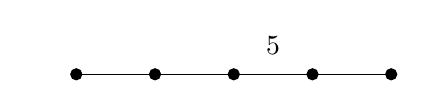
\begin{tikzpicture}[scale=1.0]
\draw[fill=black] \foreach \x in {1,2,...,5} {(\x,1.5) circle (2pt)};%\widetilde{F}_{4}
\draw {(.5,1.5) node{}
(3.5,1.5) node[label=above:$5$]{}
[-] (1,1.5) -- (5,1.5)
(2,1.5) node{}}; 
\end{tikzpicture}
\caption{$\widetilde{F}_{4}$} \label{fig:H}
\end{subfigure} &

\begin{subfigure}{0.5\textwidth} \centering
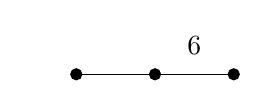
\begin{tikzpicture}[scale=1.0]
\draw[fill=black] \foreach \x in {1,2,...,3} {(\x,1.5) circle (2pt)};%\widetilde{G}_{2}
\draw {(.5,1.5) node{}
(2.5,1.5) node[label=above:$6$]{}
[-] (1,1.5) -- (3,1.5)
(2,1.5) node{}}; 
\end{tikzpicture}
\caption{$\widetilde{G}_{4}$} \label{fig:H}
\end{subfigure}
\end{tabular}
\caption{Coxeter graphs corresponding to the infinite Coxeter groups}
\label{fig:infincoxgraphs}
\end{figure}

\newpage
FC-finite Coxeter Groups
\begin{figure}[h!]
\begin{tabular}{m{7cm} m{7cm}}
\begin{subfigure}{0.5\textwidth} \centering
\begin{tikzpicture}[scale=1.0]%A_{n}
\draw[fill=black] \foreach \x in {1,2,...,6} {(\x,10) circle (2pt)};
\draw {(.5,10) node{}
(1.5,10) node[label=above:\textcolor{white}{$4$}]{}
(4.5,10) node{$\cdots$}
[-] (1,10) -- (4,10)
[-] (5,10) -- (6,10)
(1,10) node{}}; 
\end{tikzpicture}
\caption{$A_{n}$} \label{fig:FCA}
\end{subfigure} &

\begin{subfigure}{0.5\textwidth} \centering
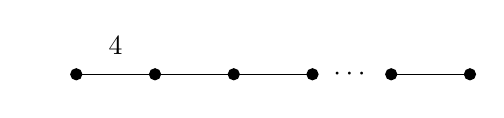
\begin{tikzpicture}[scale=1.0]%B_{n}
\draw [fill=black] \foreach \x in {1,2,...,6} {(\x,8.5) circle (2pt)};
\draw {(.5,8.5) node{}
(1.5,8.5) node[label=above:$4$]{}
(4.5,8.5) node{$\cdots$}
[-] (1,8.5) -- (4,8.5)
[-] (5,8.5) -- (6,8.5)
(2,8.5) node{}}; 
\end{tikzpicture}
\caption{$B_{n}$} \label{fig:FCB}
\end{subfigure} \\

    & \\ 

\begin{subfigure}{0.5\textwidth} \centering
\begin{tikzpicture}[scale=1.0]
\draw[fill=black] \foreach \x in {1,2,...,6} {(\x,6.5) circle (2pt)};%D_{n}
\draw[fill=black] (2,7.5) circle (2pt);
\draw {(.5,6.5) node{}
(4.5,6.5) node{$\cdots$}
[-] (1,6.5) -- (4,6.5)
[-] (5,6.5) -- (6,6.5)
[-] (2,6.5) -- (2,7.5)
(2,6.5) node{}};
\end{tikzpicture}
\caption{$D_{n}$} \label{fig:D}
\end{subfigure} &
    
\begin{subfigure}{0.5\textwidth} \centering
\begin{tikzpicture}[scale=1.0]%E_{6}
\draw[fill=black] \foreach \x in {1,2,...,6} {(\x,4.5) circle (2pt)};
\draw[fill=black] (3,5.5) circle (2pt);
%\fill[white] (3,5.9) circle (2pt);
\draw {(.5, 4.5) node{}
(4.5,4.5) node{$\cdots$}
[-] (1,4.5) -- (4,4.5)
[-] (5,4.5) -- (6,4.5)
[-] (3,4.5) -- (3,5.5)
(3,4.5) node{}};
\end{tikzpicture}
\caption{$E_{n}$} \label{fig:En}
\end{subfigure} \\

&\\

\begin{subfigure}{0.5\textwidth} \centering
\begin{tikzpicture}[scale=1.0]%F_{n}
\draw[fill=black] \foreach \x in {1,2,...,6} {(\x,3) circle (2pt)};
\fill[white] (1,4) circle (2pt);
\draw {(.5,3) node{}
(2.5,3) node[label=above:$4$]{}
(4.5,3) node{$\cdots$}
[-] (1,3) -- (4,3)
[-] (5,3) -- (6,3)
(3,3) node{}};
\end{tikzpicture}
\caption{$F_{n}$} \label{fig:Fn}
\end{subfigure} &


\begin{subfigure}{0.5\textwidth} \centering
\begin{tikzpicture}[scale=1.0]
\draw[fill=black] \foreach \x in {1,2,...,6} {(\x,1.5) circle (2pt)};%H_{4}
\fill[white] (1,3) circle (2pt);
\draw {(.5,1.5) node{}
(1.5,1.5) node[label=above:$5$]{}
(4.5,1.5) node{$\cdots$}
[-] (1,1.5) -- (4,1.5)
[-] (5,1.5) -- (6,1.5)
(2,1.5) node{}}; 
\end{tikzpicture}
\caption{$H_{n}$} \label{fig:H}
\end{subfigure}
\end{tabular}
\caption{Coxeter graphs corresponding to the FC-finite Coxeter groups.}
\label{fig:FCfincoxgraphs}
\end{figure}



\newpage
Star Reducible Heaps
\begin{figure}[h!]
\begin{tabular}{m{7cm} m{7cm}}
\begin{subfigure}{0.5\textwidth} \centering
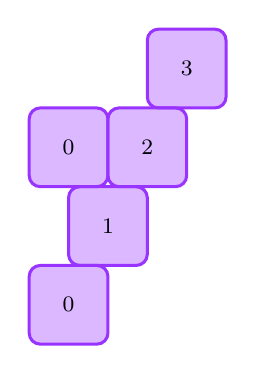
\begin{tikzpicture}[scale=0.5]
\heapblock{3}{6}{3}{purple}
\heapblock{2}{4}{2}{purple}
\heapblock{0}{4}{0}{purple}
\heapblock{1}{2}{1}{purple}
\heapblock{0}{0}{0}{purple}
\end{tikzpicture}
\caption{\textcolor{red}{I don't know what to call this}} \label{fig:heapy}
\end{subfigure} &

\begin{subfigure}{0.5\textwidth} \centering
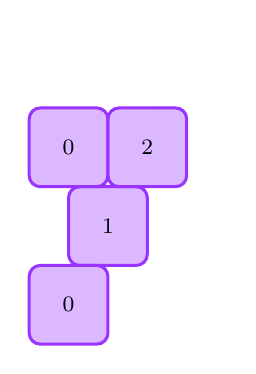
\begin{tikzpicture}[scale=0.5]
\heapblock{3}{6}{}{white}
\heapblock{2}{4}{2}{purple}
\heapblock{0}{4}{0}{purple}
\heapblock{1}{2}{1}{purple}
\heapblock{0}{0}{0}{purple}
\end{tikzpicture}
\caption{\textcolor{red}{I don't know what to call this}} \label{fig:multiplied}
\end{subfigure}
\end{tabular}
\caption{Visualization of Example~\ref{ex:starred}}
\label{fig:starred}
\end{figure}


Weak Star Reducible Heap\\
\begin{figure}
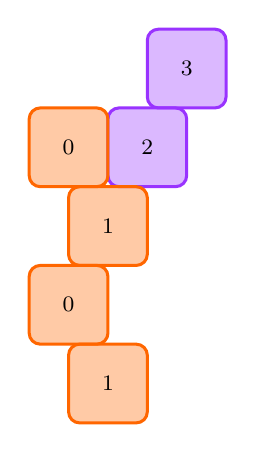
\begin{tikzpicture}[scale=0.5]
\heapblock{3}{6}{3}{purple}
\heapblock{2}{4}{2}{purple}
\heapblock{0}{4}{0}{orange}
\heapblock{1}{2}{1}{orange}
\heapblock{0}{0}{0}{orange}
\heapblock{1}{-2}{1}{orange}
\end{tikzpicture}
\caption{\textcolor{red}{I don't know what to call this}} \label{fig:noncancel}
\end{figure}


\newpage



Heaps for Property-T Section\\

\begin{figure}[h!]
\begin{tabular}{m{7cm} m{7cm}}
\begin{subfigure}{0.5\textwidth} \centering
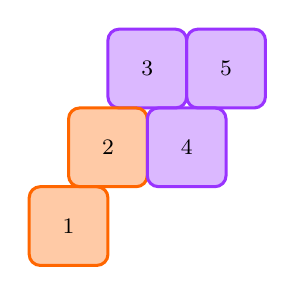
\begin{tikzpicture}[scale=0.5]
\heapblock{5}{6}{5}{purple}
\heapblock{3}{6}{3}{purple}
\heapblock{2}{4}{2}{orange}
\heapblock{4}{4}{4}{purple}
\heapblock{1}{2}{1}{orange}
\end{tikzpicture}
\caption{Heap of an element with Property-T} \label{fig:heapw/T}	
\end{subfigure}&

\begin{subfigure}{0.5\textwidth} \centering
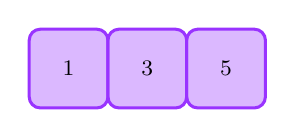
\begin{tikzpicture}[scale=0.5]
\heapblock{1}{6}{1}{purple}
\heapblock{3}{6}{3}{purple}
\heapblock{5}{6}{5}{purple}
\end{tikzpicture}
\caption{Heap of a T-Avoiding element}\label{fig:heapnoT}
\end{subfigure}
\end{tabular}
\caption{Heaps of an element with Property-T and a T-Avoiding element}
\end{figure}

\begin{figure}
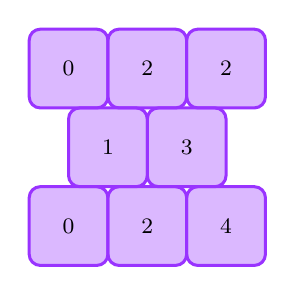
\begin{tikzpicture}[scale=0.5]
\heapblock{0}{6}{0}{purple}
\heapblock{2}{6}{2}{purple}
\heapblock{4}{6}{2}{purple}
\heapblock{1}{4}{1}{purple}
\heapblock{3}{4}{3}{purple}
\heapblock{0}{2}{0}{purple}
\heapblock{2}{2}{2}{purple}
\heapblock{4}{2}{4}{purple}
\end{tikzpicture}
\caption{Heap of a non-trivially T-Avoiding element in $W(\widetilde{C}_4)$.}	
\end{figure}


\newpage
Impermissible subheaps for elements in FC groups

\begin{figure}[h!]
\begin{tabular}{m{4cm} m{4cm} m{4cm}}
	\begin{subfigure}{0.33\textwidth} \centering
	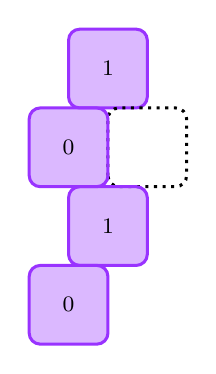
\begin{tikzpicture}[scale=0.5]
		\heapblock{1}{6}{1}{purple}
		\dheapblock{2}{4}{}{black}
		\heapblock{0}{4}{0}{purple}
		\heapblock{1}{2}{1}{purple}
		\heapblock{0}{0}{0}{purple}
	\end{tikzpicture}
	\caption{}\label{fig:C&B}
	\end{subfigure} &
	
	\begin{subfigure}{0.33\textwidth} \centering
	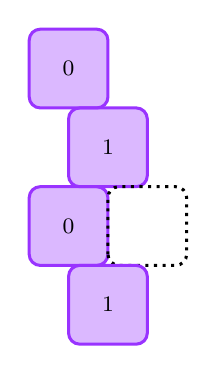
\begin{tikzpicture}[scale=0.5]
		\heapblock{0}{6}{0}{purple}
		\heapblock{1}{4}{1}{purple}
		\heapblock{0}{2}{0}{purple}
		\dheapblock{2}{2}{}{black}
		\heapblock{1}{0}{1}{purple}
	\end{tikzpicture}
	\caption{}\label{fig:C&B2}
	\end{subfigure} &

	\begin{subfigure} {0.33\textwidth} \centering
	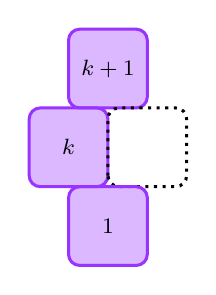
\begin{tikzpicture}[scale=0.5]
		\heapblock{1}{6}{k+1}{purple}
		\heapblock{0}{4}{k}{purple}
		\dheapblock{2}{4}{}{black}
		\heapblock{1}{2}{1}{purple}
	\end{tikzpicture}
	\caption{}\label{fig:a,b,c}
	\end{subfigure}\\
	
	&\\
	
	\begin{subfigure}{0.33\textwidth} \centering
	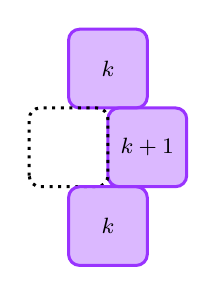
\begin{tikzpicture}[scale=0.5]
		\heapblock{2}{6}{k}{purple}
		\heapblock{3}{4}{k+1}{purple}
		\dheapblock{1}{4}{}{black}
		\heapblock{2}{2}{k}{purple}
	\end{tikzpicture}
	\caption{}\label{fig:a,b,c2}
	\end{subfigure}&
	
	\begin{subfigure}{0.33\textwidth} \centering
	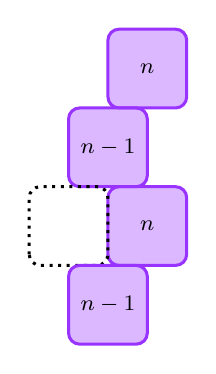
\begin{tikzpicture}[scale=0.5]
		\heapblock{2}{6}{n}{purple}
		\heapblock{1}{4}{n-1}{purple}
		\heapblock{2}{2}{n}{purple}
		\dheapblock{0}{2}{}{black}
		\heapblock{1}{0}{n-1}{purple}
	\end{tikzpicture}
	\caption{}\label{fig:cimpermiss}	
	\end{subfigure} &
	
	\begin{subfigure}{0.33\textwidth} \centering
	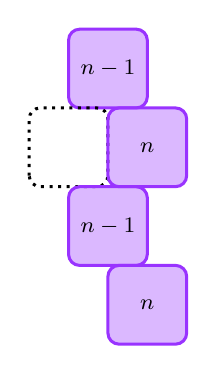
\begin{tikzpicture}[scale=0.5]
		\heapblock{1}{6}{n-1}{purple}
		\dheapblock{0}{4}{}{black}
		\heapblock{2}{4}{n}{purple}
		\heapblock{1}{2}{n-1}{purple}
		\heapblock{2}{0}{n}{purple}
	\end{tikzpicture}	
	\caption{}\label{fig:cimpermiss2}
	\end{subfigure}
\end{tabular}	
\caption{Impermissible subheaps for elements in FC$(\widetilde{C}_n)$.}\label{fig:impermiss heaps}
\end{figure}


\begin{figure}
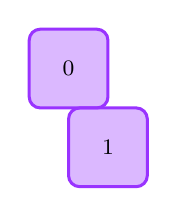
\begin{tikzpicture}[scale=0.5]
\heapblock{0}{2}{0}{purple}
\heapblock{1}{0}{1}{purple}	
\end{tikzpicture}	
\end{figure}

\begin{figure*}
\begin{tabular}{m{4cm} m{4cm}}
\begin{subfigure}{0.5\textwidth} \centering
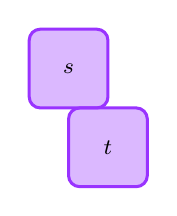
\begin{tikzpicture}[scale=0.5]
	\heapblock{0}{2}{s}{purple}
	\heapblock{1}{0}{t}{purple}
\end{tikzpicture}

(reduced product)
\caption{}
\end{subfigure} &

\begin{subfigure}{0.5\textwidth} \centering
(reduced product)

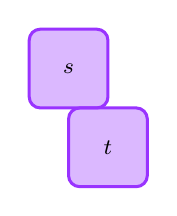
\begin{tikzpicture}[scale=0.5]
	\heapblock{0}{2}{s}{purple}
	\heapblock{1}{0}{t}{purple}
\end{tikzpicture}
\caption{}	
\end{subfigure}
\end{tabular}
\caption{A visual representation of Property T.}\label{heapwithT}
\end{figure*}

\newpage

Single Bowtie

\begin{figure*}[h!]
\begin{tabular}{m{4cm} m{4cm}}
\begin{subfigure}{0.5\textwidth} \centering
\begin{tikzpicture}[scale=0.5]
	\heapblock{1}{10}{1}{purple}
	\heapblock{3}{10}{3}{orange}
	\heapblock{5}{10}{5}{purple}
	\heapblock{2}{8}{2}{orange}
	\heapblock{4}{8}{4}{purple}
	\heapblock{3}{6}{3}{orange}
	\heapblock{2}{4}{2}{orange}
	\heapblock{4}{4}{4}{purple}
	\heapblock{1}{2}{1}{purple}
	\heapblock{3}{2}{3}{orange}
	\heapblock{5}{2}{5}{purple}
\end{tikzpicture}
\caption{}\label{fig:singbowtie4}
\end{subfigure}&

\begin{subfigure}{0.5\textwidth}\centering
\begin{tikzpicture}[scale=0.5]
	\heapblock{1}{10}{1}{purple}
	\heapblock{3}{10}{3}{purple}
	\heapblock{5}{10}{5}{purple}
	\heapblock{2}{8}{2}{purple}
	\heapblock{4}{8}{4}{teal}
	\heapblock{3}{6}{3}{teal}
	\heapblock{2}{4}{2}{purple}
	\heapblock{4}{4}{4}{teal}
	\heapblock{1}{2}{1}{purple}
	\heapblock{3}{2}{3}{purple}
	\heapblock{5}{2}{5}{purple}
\end{tikzpicture}
\caption{}\label{fig:singbowtiebraid}
\end{subfigure}
\end{tabular}
\caption{A single bowtie in $W(F_5)$.}\label{fig:singbowtie}	
\end{figure*}

\begin{figure*}[h!]
\begin{tikzpicture}[scale=0.5]
\heapblock{1}{10}{1}{purple}
	\heapblock{3}{10}{3}{orange}
	\heapblock{5}{10}{5}{purple}
	\heapblock{2}{8}{2}{orange}
	\heapblock{4}{8}{4}{purple}
	\heapblock{3}{6}{3}{orange}
	\heapblock{2}{4}{2}{orange}
	\heapblock{4}{4}{4}{purple}
	\heapblock{1}{2}{1}{purple}
	\heapblock{3}{2}{3}{orange}
	\heapblock{5}{2}{5}{purple}
	\heapblock{2}{0}{2}{orange}
	\heapblock{4}{0}{4}{purple}
	\heapblock{3}{-2}{3}{orange}
	\heapblock{2}{-4}{2}{orange}
	\heapblock{4}{-4}{4}{purple}
	\heapblock{1}{-6}{1}{purple}
	\heapblock{3}{-6}{3}{orange}
	\heapblock{5}{-6}{5}{purple}
	
	\node[] at (3,-8){$\vdots$};
	
	\heapblock{1}{-10}{1}{purple}
	\heapblock{3}{-10}{3}{orange}
	\heapblock{5}{-10}{5}{purple}
	\heapblock{2}{-12}{2}{orange}
	\heapblock{4}{-12}{4}{purple}
	\heapblock{3}{-14}{3}{orange}
	\heapblock{2}{-16}{2}{orange}
	\heapblock{4}{-16}{4}{purple}
	\heapblock{1}{-18}{1}{purple}
	\heapblock{3}{-18}{3}{orange}
	\heapblock{5}{-18}{5}{purple}
\end{tikzpicture}
\caption{A stack of bowties in $W(F_5)$.}\label{fig:stackobowties}
\end{figure*}

\begin{figure}[h!]\centering
\begin{tikzpicture}[scale=0.5]
	\heapblock{2}{10}{2}{orange}
	\heapblock{4}{10}{4}{purple}
	\heapblock{6}{10}{6}{purple}
	\heapblock{3}{8}{3}{orange}
	\heapblock{5}{8}{5}{purple}
	\heapblock{2}{6}{2}{orange}
	\heapblock{4}{6}{4}{purple}
	\heapblock{1}{4}{1}{purple}
	\heapblock{3}{4}{3}{orange}
	\heapblock{2}{2}{2}{orange}
	\heapblock{1}{0}{1}{purple}
	\heapblock{3}{0}{3}{orange}
	\heapblock{2}{-2}{2}{orange}
	\heapblock{4}{-2}{4}{purple}
	\heapblock{3}{-4}{3}{orange}
	\heapblock{5}{-4}{5}{purple}
	\heapblock{2}{-6}{2}{orange}
	\heapblock{4}{-6}{4}{purple}
	\heapblock{6}{-6}{6}{purple}
\end{tikzpicture}
\caption{A non-trivial T-avoiding element in $W(F_6)$}\label{fig:f6bat}
\end{figure}

Labeled Coxeter Graphs that the thesis deals with

\begin{figure}[h!]
\begin{tabular}{m{7cm} m{7cm}}
\begin{subfigure}{0.5\textwidth} \centering
\begin{tikzpicture}[scale=1.0]%A_{n}
\draw[fill=black] \foreach \x in {1,2,...,6} {(\x,10) circle (2pt)};
\draw {(.5,10) node{}
(1.5,10) node[label=above:\textcolor{white}{$4$}]{}
(4.5,10) node{$\cdots$}
(1,10) node[label=below:$s_1$]{}
(2,10) node[label=below:$s_2$]{}
(3,10) node[label=below:$s_3$]{}
(4,10) node[label=below:$s_4$]{}
(5,10) node[label=below:$s_{n-1}$]{}
(6,10) node[label=below:$s_{n}$]{}
[-] (1,10) -- (4,10)
[-] (5,10) -- (6,10)
(1,10) node{}}; 
\end{tikzpicture}
\caption{$A_{n}$} \label{fig:labeledA}
\end{subfigure} &

\begin{subfigure}{0.5\textwidth} \centering
\begin{tikzpicture}[scale=1.0]%\widetilde{A}_{n}
\draw [fill=black] \foreach \x in {1,...,4} {(\x,7.5) circle (2pt)};
\draw [fill=black] (2.5, 8.5) circle (2pt);
\draw {(.5,8.5) node{}
(2.5,7.5) node{$\cdots$}
(1,7.5) node[label=below:$s_1$]{}
(2,7.5) node[label=below:$s_2$]{}
(3,7.5) node[label=below:$s_{n-1}$]{}
(4,7.5) node[label=below:$s_{n}$]{}
(2.5,8.5) node[label=right:$s_{n+1}$]{}
[-] (2.5,8.5) -- (1, 7.5)
[-] (2.5,8.5) -- (4, 7.5)
[-] (1,7.5) -- (2,7.5)
[-] (3,7.5) -- (4,7.5)
(2,8.5) node{}}; 
\end{tikzpicture}
\caption{$\widetilde{A}_{n}$} \label{fig:labeledaffAn}
\end{subfigure} \\

    & \\ 

\begin{subfigure}{0.5\textwidth} \centering
\begin{tikzpicture}[scale=1.0]%B_{n}
\draw [fill=black] \foreach \x in {1,2,...,6} {(\x,8.5) circle (2pt)};
\draw {(.5,8.5) node{}
(1.5,8.5) node[label=above:$4$]{}
(4.5,8.5) node{$\cdots$}
(1,8.5) node[label=below:$s_0$]{}
(2,8.5) node[label=below:$s_1$]{}
(3,8.5) node[label=below:$s_2$]{}
(4,8.5) node[label=below:$s_3$]{}
(5,8.5) node[label=below:$s_{n-2}$]{}
(6,8.5) node[label=below:$s_{n-1}$]{}
[-] (1,8.5) -- (4,8.5)
[-] (5,8.5) -- (6,8.5)
(2,8.5) node{}}; 
\end{tikzpicture}
\caption{$B_{n}$} \label{fig:labeledB}
\end{subfigure} &

\begin{subfigure}{0.5\textwidth} \centering
\begin{tikzpicture}[scale=1.0]
\draw[fill=black] \foreach \x in {1,2,...,6} {(\x,5) circle (2pt)};%\widetild{C}_{n}
\fill[white] (1,6) circle (2pt);
\draw {(.5,5) node{}
(4.5,5) node{$\cdots$}
(5.5,5) node[label=above:$4$]{}
(1.5,5) node[label=above:$4$]{}
(1,5) node[label=below:$s_0$]{}
(2,5) node[label=below:$s_1$]{}
(3,5) node[label=below:$s_2$]{}
(4,5) node[label=below:$s_3$]{}
(5,5) node[label=below:$s_{n-1}$]{}
(6,5) node[label=below:$s_{n}$]{}
[-] (1,5) -- (4,5)
[-] (5,5) -- (6,5)
(2,5) node{}};
\end{tikzpicture}
\caption{$\widetilde{C}_{n}$} \label{fig:labeledaffC}
\end{subfigure}  \\

& \\

\begin{subfigure}{0.5\textwidth} \centering
\begin{tikzpicture}[scale=1.0]
\draw[fill=black] \foreach \x in {1,2,...,6} {(\x,6.5) circle (2pt)};%D_{n}
\draw[fill=black] (2,7.5) circle (2pt);
\draw {(.5,6.5) node{}
(4.5,6.5) node{$\cdots$}
(1,6.5) node[label=below:$s_1$]{}
(2,6.5) node[label=below:$s_2$]{}
(3,6.5) node[label=below:$s_3$]{}
(4,6.5) node[label=below:$s_4$]{}
(5,6.5) node[label=below:$s_{n-2}$]{}
(6,6.5) node[label=below:$s_{n-1}$]{}
(2,7.5) node[label=right:$s_0$]{}
[-] (1,6.5) -- (4,6.5)
[-] (5,6.5) -- (6,6.5)
[-] (2,6.5) -- (2,7.5)
(2,6.5) node{}};
\end{tikzpicture}
\caption{$D_{n}$} \label{fig:labeledD}
\end{subfigure}&

\begin{subfigure}{0.5\textwidth} \centering
\begin{tikzpicture}[scale=1.0]%F_{n}
\draw[fill=black] \foreach \x in {1,2,...,6} {(\x,3) circle (2pt)};
\fill[white] (1,4) circle (2pt);
\draw {(.5,3) node{}
(2.5,3) node[label=above:$4$]{}
(4.5,3) node{$\cdots$}
(1,3) node[label=below:$s_1$]{}
(2,3) node[label=below:$s_2$]{}
(3,3) node[label=below:$s_3$]{}
(4,3) node[label=below:$s_4$]{}
(5,3) node[label=below:$s_{n-1}$]{}
(6,3) node[label=below:$s_{n}$]{}
[-] (1,3) -- (4,3)
[-] (5,3) -- (6,3)
(3,3) node{}};
\end{tikzpicture}
\caption{$F_{n}$} \label{fig:labeledFn}
\end{subfigure}  \\

& \\

\begin{subfigure}{0.5\textwidth} \centering
\begin{tikzpicture}[scale=1.0]
\draw[fill=black] \foreach \x in {1,2} {(\x,0) circle (2pt)};
\fill[fill=white] (2,1) circle (2pt);
\draw {(.25,0) node{}
(1.5,0) node[label=above:$m$]{}
(1,0) node[label=below:$s_1$]{}
(2,0) node[label=below:$s_2$]{}
[-] (1,0) -- (2,0)
(2,0) node{}};
\end{tikzpicture}
\caption{$I_{2}(m)$} \label{fig:labeledI}
\end{subfigure}
\end{tabular}
\caption{Labeled Coxeter Graphs}\label{}
\end{figure}

\begin{figure}[h!]
\begin{tabular}{m{7cm} m{7cm}}
\begin{subfigure}{0.5\textwidth} \centering
\begin{tikzpicture}[scale=0.5]
	\heapblock{3}{-2}{}{white}
	\heapblock{2}{6}{k}{teal}
	\heapblock{3}{4}{k-1}{teal}
	\heapblock{2}{2}{k}{teal}
	\heapblock{4}{2}{k-2}{purple}
	\heapblock{3}{0}{k-1}{purple}
\end{tikzpicture}
\caption{}\label{case:a1}
\end{subfigure}&

\begin{subfigure}{0.5\textwidth} \centering
\begin{tikzpicture}[scale=0.5]
	\heapblock{3}{8}{k-1}{purple}
	\heapblock{2}{6}{k}{purple}
	\heapblock{3}{4}{k-1}{teal}
	\heapblock{4}{2}{k-2}{teal}
	\heapblock{3}{0}{k-1}{teal}
\end{tikzpicture}
\caption{}\label{case:a2}
\end{subfigure}	
\end{tabular}
\caption{Visual representation of the heap configuration discussed in Case 1a.}
\end{figure}

\begin{figure}[h!]
\begin{tabular}{m{7cm} m{7cm}}
\begin{subfigure}{0.5\textwidth} \centering
\begin{tikzpicture}[scale=0.5]
	\heapblock{4}{4}{k}{teal}
	\heapblock{3}{2}{k-1}{teal}
	\dheapblock{2}{0}{}{black}
	\heapblock{4}{0}{k}{teal}
	\dheapblock{3}{-2}{}{black}
	\heapblock{5}{-2}{k+1}{purple}
\end{tikzpicture}
\caption{}\label{fig:caseb1}
\end{subfigure} &

\begin{subfigure}{0.5\textwidth} \centering
\begin{tikzpicture}[scale=0.5]
	\heapblock{3}{6}{}{white}
	\heapblock{3}{4}{k-1}{teal}
	\heapblock{4}{2}{k}{teal}
	\dheapblock{2}{2}{}{black}
	\heapblock{3}{0}{k-1}{teal}
	\heapblock{5}{0}{k+1}{purple}
\end{tikzpicture}
\caption{}\label{fig:caseb2}
\end{subfigure}
\end{tabular}
\caption{Visual representation of the heap configuration discussed in Case 1b.}\label{fig:Case1b}
\end{figure}

\begin{figure}[h!]
\begin{tabular}{m{7cm} m{7cm}}
\begin{subfigure}{0.5\textwidth} \centering
\begin{tikzpicture}[scale=0.5]
	\heapblock{0}{-2}{}{white}
	\heapblock{2}{8}{2}{teal}
	\heapblock{1}{6}{1}{teal}
	\heapblock{2}{4}{2}{teal}
	\heapblock{0}{4}{0}{purple}
	\heapblock{1}{2}{1}{purple}
	\heapblock{0}{0}{0}{purple}
	\dheapblock{2}{0}{}{black}
\end{tikzpicture}
\caption{}\label{fig:case2b1}
\end{subfigure} &

\begin{subfigure}{0.5\textwidth} \centering
\begin{tikzpicture}[scale=0.5]
	\heapblock{1}{8}{1}{purple}
	\heapblock{2}{6}{2}{purple}
	\heapblock{1}{4}{1}{orange}
	\heapblock{0}{2}{0}{orange}
	\heapblock{1}{0}{1}{orange}
	\heapblock{0}{-2}{0}{orange}
	\dheapblock{2}{-2}{}{black}
\end{tikzpicture}
\caption{}\label{fig:case2b2}
\end{subfigure}
\end{tabular}
\caption{Visual representation of the heap configuration discussed in Case 2a.}\label{fig:Case2a}
\end{figure}

\begin{figure}[h!]
\begin{tabular}{m{7cm} m{7cm}}
\begin{subfigure}{0.5\textwidth} \centering
\begin{tikzpicture}[scale=0.5]
	\heapblock{0}{10}{0}{orange}
	\heapblock{1}{8}{1}{orange}
	\heapblock{0}{6}{0}{orange}
	\heapblock{1}{4}{1}{orange}
	\heapblock{2}{2}{2}{purple}
	\dheapblock{0}{2}{}{black}
\end{tikzpicture}
\caption{}\label{fig:case3a1}
\end{subfigure} &

\begin{subfigure}{0.5\textwidth} \centering
\begin{tikzpicture}[scale=0.5]
	\heapblock{0}{12}{}{white}
	\heapblock{1}{10}{1}{orange}
	\heapblock{0}{8}{0}{orange}
	\heapblock{1}{6}{1}{orange}
	\heapblock{0}{4}{0}{orange}
	\heapblock{2}{4}{2}{purple}
\end{tikzpicture}
\caption{}\label{fig:case3a2}
\end{subfigure}
\end{tabular}
\caption{Visual representation of the heap configuration discussed in Case 3a.}\label{fig:Case3a}
\end{figure}

\begin{figure}[h!]
\begin{tabular}{m{7cm} m{7cm}}
\begin{subfigure}{0.5\textwidth} \centering
\begin{tikzpicture}[scale=0.5]
	\heapblock{1}{8}{1}{teal}
	\heapblock{2}{6}{2}{teal}
	\heapblock{1}{4}{1}{teal}
	\heapblock{0}{2}{0}{purple}
	\dheapblock{2}{2}{}{black}
\end{tikzpicture}
\caption{}\label{fig:case3b1}
\end{subfigure} &

\begin{subfigure}{0.5\textwidth} \centering
\begin{tikzpicture}[scale=0.5]
	\heapblock{0}{8}{}{white}
	\heapblock{2}{6}{2}{teal}
	\heapblock{1}{4}{1}{teal}
	\heapblock{2}{2}{2}{teal}
	\heapblock{0}{2}{0}{purple}
\end{tikzpicture}
\caption{}\label{fig:case3b2}
\end{subfigure}
\end{tabular}
\caption{Visual representation of the heap configuration discussed in Case 3b.}\label{fig:Case3b}
\end{figure}

\begin{figure}[h!]
\begin{tabular}{m{7cm} m{7cm}}
\begin{subfigure}{0.5\textwidth} \centering
\begin{tikzpicture}[scale=0.5]
	\heapblock{0}{0}{}{white}
	\heapblock{1}{10}{1}{orange}
	\heapblock{0}{8}{0}{orange}
	\heapblock{1}{6}{1}{orange}
	\heapblock{0}{4}{0}{orange}
	\heapblock{2}{4}{2}{purple}
	\heapblock{1}{2}{1}{purple}
\end{tikzpicture}
\caption{}\label{fig:case4a}
\end{subfigure} &

\begin{subfigure}{0.5\textwidth} \centering
\begin{tikzpicture}[scale=0.5]
	\heapblock{0}{10}{0}{orange}
	\heapblock{1}{8}{1}{orange}
	\heapblock{0}{6}{0}{orange}
	\heapblock{1}{4}{1}{teal}
	\heapblock{2}{2}{2}{teal}
	\heapblock{1}{0}{1}{teal}
\end{tikzpicture}
\caption{}\label{fig:case4b}
\end{subfigure}
\end{tabular}
\caption{Visual representation of the heap configuration discussed in Case 4.}\label{fig:Case4}
\end{figure}

\begin{figure}[h!]
\begin{tabular}{m{7cm} m{7cm}}
\begin{subfigure}{0.5\textwidth} \centering
\begin{tikzpicture}[scale=0.5]
	\heapblock{0}{12}{}{white}
	\heapblock{2}{10}{2}{teal}
	\heapblock{1}{8}{1}{teal}
	\heapblock{2}{6}{2}{teal}
	\heapblock{0}{6}{0}{purple}
	\heapblock{1}{4}{1}{purple}
	\heapblock{3}{4}{3}{purple}
\end{tikzpicture}
\caption{}\label{fig:caseb2a}
\end{subfigure} &

\begin{subfigure}{0.5\textwidth} \centering
\begin{tikzpicture}[scale=0.5]
	\heapblock{1}{10}{1}{teal}
	\heapblock{2}{8}{2}{teal}
	\heapblock{1}{6}{1}{teal}
	\heapblock{0}{4}{0}{purple}
	\heapblock{1}{2}{1}{purple}
	\heapblock{3}{2}{3}{purple}
\end{tikzpicture}
\caption{}\label{fig:caseb2b}
\end{subfigure}
\end{tabular}
\caption{Visual representation of the heap configuration discussed in Case 2b.}\label{fig:Case2}
\end{figure}

\begin{figure} \centering
\begin{tikzpicture}[scale=0.5] 
	\heapblock{2}{10}{2}{teal}
	\heapblock{1}{8}{1}{teal}
	\heapblock{2}{6}{2}{teal}
	\heapblock{0}{6}{0}{purple}
	\heapblock{1}{4}{1}{purple}
	\heapblock{3}{4}{3}{purple}
	\heapblock{2}{2}{2}{rred}
\end{tikzpicture}\label{heap2}
\end{figure}

\begin{figure} \centering
\begin{tikzpicture}[scale=0.5] 
	\heapblock{2}{10}{2}{teal}
	\heapblock{1}{8}{1}{teal}
	\heapblock{2}{6}{2}{teal}
	\heapblock{0}{6}{0}{purple}
	\heapblock{1}{4}{1}{purple}
	\heapblock{3}{4}{3}{purple}
	\heapblock{2}{2}{2}{rred}
	\heapblock{3}{0}{3}{rred}
	\heapblock{4}{2}{4}{rred}
\end{tikzpicture}\label{heap2}
\end{figure}

\begin{figure} \centering
\begin{tikzpicture}[scale=0.5] 
	\heapblock{2}{10}{2}{teal}
	\heapblock{1}{8}{1}{teal}
	\heapblock{2}{6}{2}{teal}
	\heapblock{0}{6}{0}{purple}
	\heapblock{1}{4}{1}{purple}
	\heapblock{3}{4}{3}{purple}
	\heapblock{2}{2}{2}{rred}
	\heapblock{3}{0}{3}{rred}
	\heapblock{4}{2}{4}{rred}
	\heapblock{5}{0}{5}{rred}
	\heapblock{4}{-2}{4}{rred}
	
	\node[] at (7,-2){$\ddots$};
	\node[] at (7,-4){$\ddots$};
	
	\heapblock{9}{-3}{n-3}{rred}
	\heapblock{11}{-3}{n-1}{rred}
	\heapblock{10}{-5}{n-2}{rred}
	\heapblock{12}{-5}{n}{rred}
	
\end{tikzpicture}\label{heap2}
\end{figure}

\begin{figure}[h!] \centering
\begin{tikzpicture}[scale=0.5] 
	\heapblock{2}{10}{2}{teal}
	\heapblock{1}{8}{1}{teal}
	\heapblock{2}{6}{2}{teal}
	\heapblock{0}{6}{0}{purple}
	\heapblock{1}{4}{1}{purple}
	\heapblock{3}{4}{3}{purple}
	\heapblock{2}{2}{2}{rred}
	\heapblock{3}{0}{3}{rred}
	\heapblock{4}{2}{4}{rred}
	\heapblock{5}{0}{5}{rred}
	\heapblock{4}{-2}{4}{rred}
	
	\node[] at (7,-2){$\ddots$};
	\node[] at (7,-4){$\ddots$};
	
	\heapblock{9}{-3}{n-3}{rred}
	\heapblock{11}{-3}{n-1}{rred}
	\heapblock{10}{-5}{n-2}{rred}
	\heapblock{12}{-5}{n}{rred}
	\heapblock{11}{-7}{n-1}{rred}
	\heapblock{9}{-7}{n-3}{rred}
	%\heapblock{10}{-7}{n-2}{rred}
	
	\node[] at (7, -7){$\iddots$};
	\node[] at (7,-9){$\iddots$};
	\node[] at (4,-5){$\vdots$};
	
	\heapblock{3}{-8}{3}{rred}
	\heapblock{1}{-8}{1}{rred}
	\heapblock{2}{-10}{2}{rred}
	\heapblock{0}{-10}{0}{rred}
	\heapblock{4}{-10}{4}{rred}
\end{tikzpicture}\label{heap2}
\end{figure}

\begin{figure}[h!] \centering
\begin{tikzpicture}[scale=0.5] 
	\heapblock{1}{12}{1}{teal}
	\heapblock{2}{10}{2}{teal}
	\heapblock{1}{8}{1}{orange}
	\heapblock{0}{6}{0}{orange}
	\heapblock{1}{4}{1}{orange}
	\heapblock{3}{4}{3}{purple}
	\heapblock{0}{2}{0}{orange}
	\heapblock{2}{2}{2}{rred}
	\heapblock{3}{0}{3}{rred}
	\heapblock{4}{2}{4}{rred}
	\heapblock{5}{0}{5}{rred}
	\heapblock{4}{-2}{4}{rred}
	
	\node[] at (7,-2){$\ddots$};
	\node[] at (7,-4){$\ddots$};
	
	\heapblock{9}{-3}{n-3}{rred}
	\heapblock{11}{-3}{n-1}{rred}
	\heapblock{10}{-5}{n-2}{rred}
	\heapblock{12}{-5}{n}{rred}
	\heapblock{11}{-7}{n-1}{rred}
	\heapblock{9}{-7}{n-3}{rred}
	%\heapblock{10}{-7}{n-2}{rred}
	
	\node[] at (7, -7){$\iddots$};
	\node[] at (7,-9){$\iddots$};
	\node[] at (0,-3){$\vdots$};
	
	\heapblock{3}{-8}{3}{rred}
	\heapblock{1}{-8}{1}{rred}
	\heapblock{2}{-10}{2}{rred}
	\heapblock{0}{-10}{0}{rred}
	\heapblock{4}{-10}{4}{rred}
\end{tikzpicture}\label{heap2}
\end{figure}

\newpage

\begin{figure}[h!] \centering
\begin{tikzpicture}[scale=0.5]
	\heapblock{1}{10}{1}{teal}
	\heapblock{3}{10}{3}{purple}
	\heapblock{2}{8}{2}{teal}
	\heapblock{1}{6}{1}{teal}
	\heapblock{0}{4}{0}{purple}
	\heapblock{1}{2}{1}{purple}
	\heapblock{3}{2}{3}{purple}
	\heapblock{0}{0}{0}{purple}
	\heapblock{2}{0}{2}{purple}
	\heapblock{4}{0}{2}{purple}	
\end{tikzpicture}	
\end{figure}


\end{document}
=======

